%!TEX root = ../Sensors_SmartConstruction.tex
% -*- root: ../Sensors_SmartConstruction.tex -*-


%!TEX root = ../construction.tex
% -*- root: ../construction.tex -*-

\section{Experimental Result}

제안하는 시스템의 사용성과 효율성을 검증하기 위하여 사용자 테스트를 수행하였다. 실험은 \cite{yeh_-site_2012,lin_using_2014}를 참고하여 설계되었다.

\subsection{Demo Case}




\subsection{Experiments Design}

% 총 30~36명의 피실험자가 실험에 참여하였다. 이중 x명은 여자였고 x명은 남자가 참여했으며, 나이는 26세부터 43세까지이다. 피실험자의 x명은 civil engineering background이고 x명은 (construction professionals with experience in computer aided engineering, software development, structural analysis and design, construction planning, construction drawing, and project management.) 이들 대부분은 도면에 대한 이해도가 높고 CAD 프로그램에 대한 경험이 많았고, 또한 kinect등 제스처 기반 시스템에 대한 경험은 없었다. 

피실험자 설명 관련 설명: 인원, 성별 및 나이 구성, background

실험은 초반 15분 동안 demonstration session을 진행하였다. demonstration session 동안, 전체 시나리오에 대한 비디오를 보여준 후, 제안하는 시스템의 사용 방법에 대하여 설명하고, 나머지 시간 동안 실제로 사용해 본 수 있도록 하였다. 이후에 비교 실험과 사용성 평가를 실시하였다. 비교 실험은 \cite{yeh_-site_2012}과 마찬가지로 제안하는 시스템과 대조군 시스템 사이의 비교실험을 적용하여 몇 가지 과제를 수행하도록 하고 수행시간을 비교하였다. 모든 실험은 비디오로 녹화되었으며, 녹화된 동영상 분석을 통하여 수행시간을 측정하였다. 

대조군에 대한 설명 (paper 기반, 모바일, 제안하는 시스템)
모바일 앱
 - Autodesk® BIM 360 Glue
 - BIMx 

비교 실험에 수행된 과업은 \cite{yeh_-site_2012}와 유사하게 설계하여 실제 건축 환경에서 문제가 되는 task를 반영하였다. 이는 건축 현장에서 건축물의 정보를 획득하고 이를 다시 건축 모델에 반영하는 일련의 과정을 반영하고 있다. 세부적인 task는 아래와 같다. 각 task는 독립적으로 수행되었으며, 새로운 task 수행 전에 5분간의 휴식 시간을 제공하였다. 실험은 이러한 각 task의 수행 시간을 측정하였다. 
Random하게 수행하게 함

\begin{enumerate}
\item Exploration: 3차원 모델을 돌려보고 특정 뷰에 있는 특징 발견하기
\item Query: 특정 층의 특정 평면도 획득
\item Legend: 건축물의 평면도에서 특정 구조물의 dimension 획득
\item Modify: 건축물의 평면도에서 특정 구조물을 다른 위치로 이동됨을 표시
\item Discussion: 원격의 관리자와 건축물의 특정 위치의 이슈 에 대하여 의견 교환
\end{enumerate}

\begin{figure}[ht!]
	\centering
    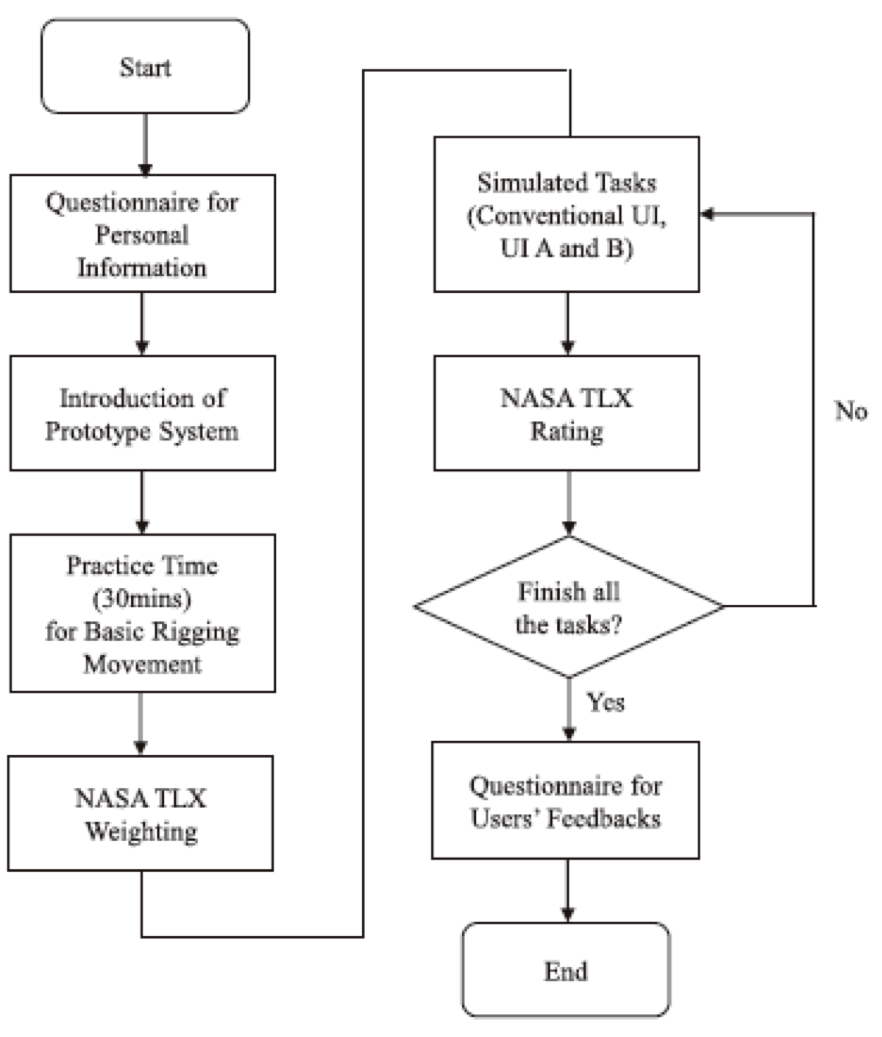
\includegraphics[width=0.4\textwidth]{5-Experiments/process}
	\caption{The process of experiments}
    \label{fig:exp_process}
\end{figure}

\ref{fig:exp_process} 와 같은 형태로 실험 단계 수행

\subsection{Efficiency}

Completion time, success rate test

\subsection{effectiveness}
Task loading score for participants (NASA Task Load indeX) test

\textit{
\begin{itemize}
\item Six weighted factors (Mental Demands, physical demands, temporal demands, effort, performance, frustration)
\item Mental Demand: How much mental and perceptual activity was required? Was the task easy or demanding, simple or complex?
\item Physical Demand: How much physical activity was required? Was the task easy or demanding, slack or strenuous?
\item Temporal Demand: How much time pressure did you feel due to the pace at which the tasks or task elements occurred? Was the pace slow or rapid?
\item Overall Performance: How successful were you in performing the task? How satisfied were you with your performance?
\item Frustration Level: How irritated, stressed, and annoyed versus content, relaxed, and complacent did you feel during the task?
\item Effort: How hard did you have to work (mentally and physically) to accomplish your level of performance?
\end{itemize}
}

\begin{figure}[ht!]
	\centering
    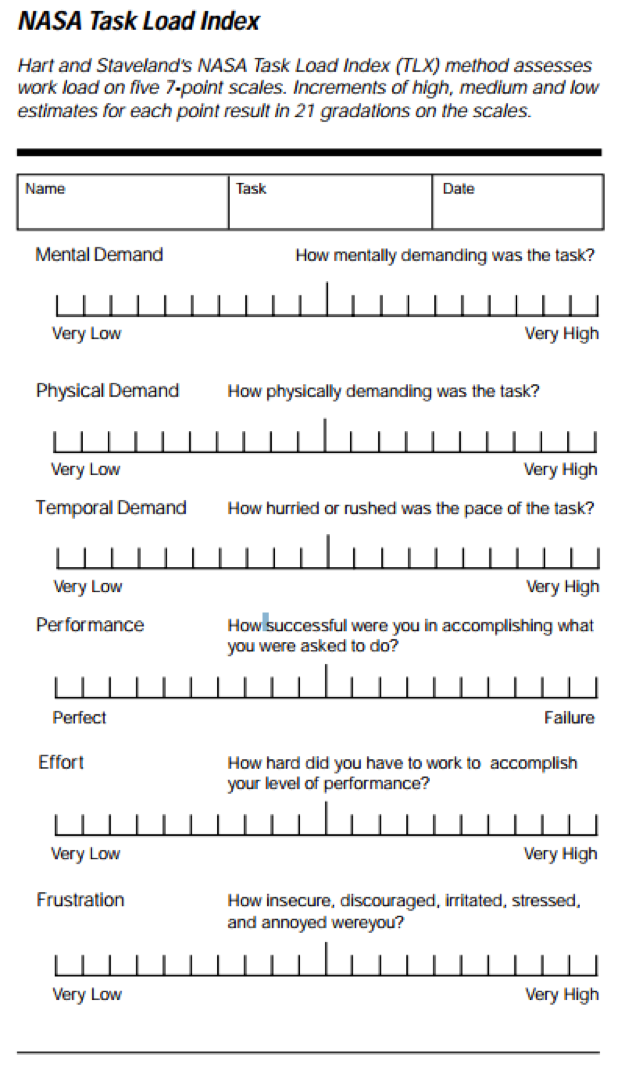
\includegraphics[width=0.4\textwidth]{5-Experiments/NASATLX}
	\caption{Questionnaire of NASA TLX}
    \label{fig:nasa_tlx}
\end{figure}

\subsection{usability}

Usability test (Perceived Usefulness and Usability)





%===============================================================================================
%	Experiments
%	목표 분량: 0.5장

%  \begin{figure*}[!t]
% \centering
% 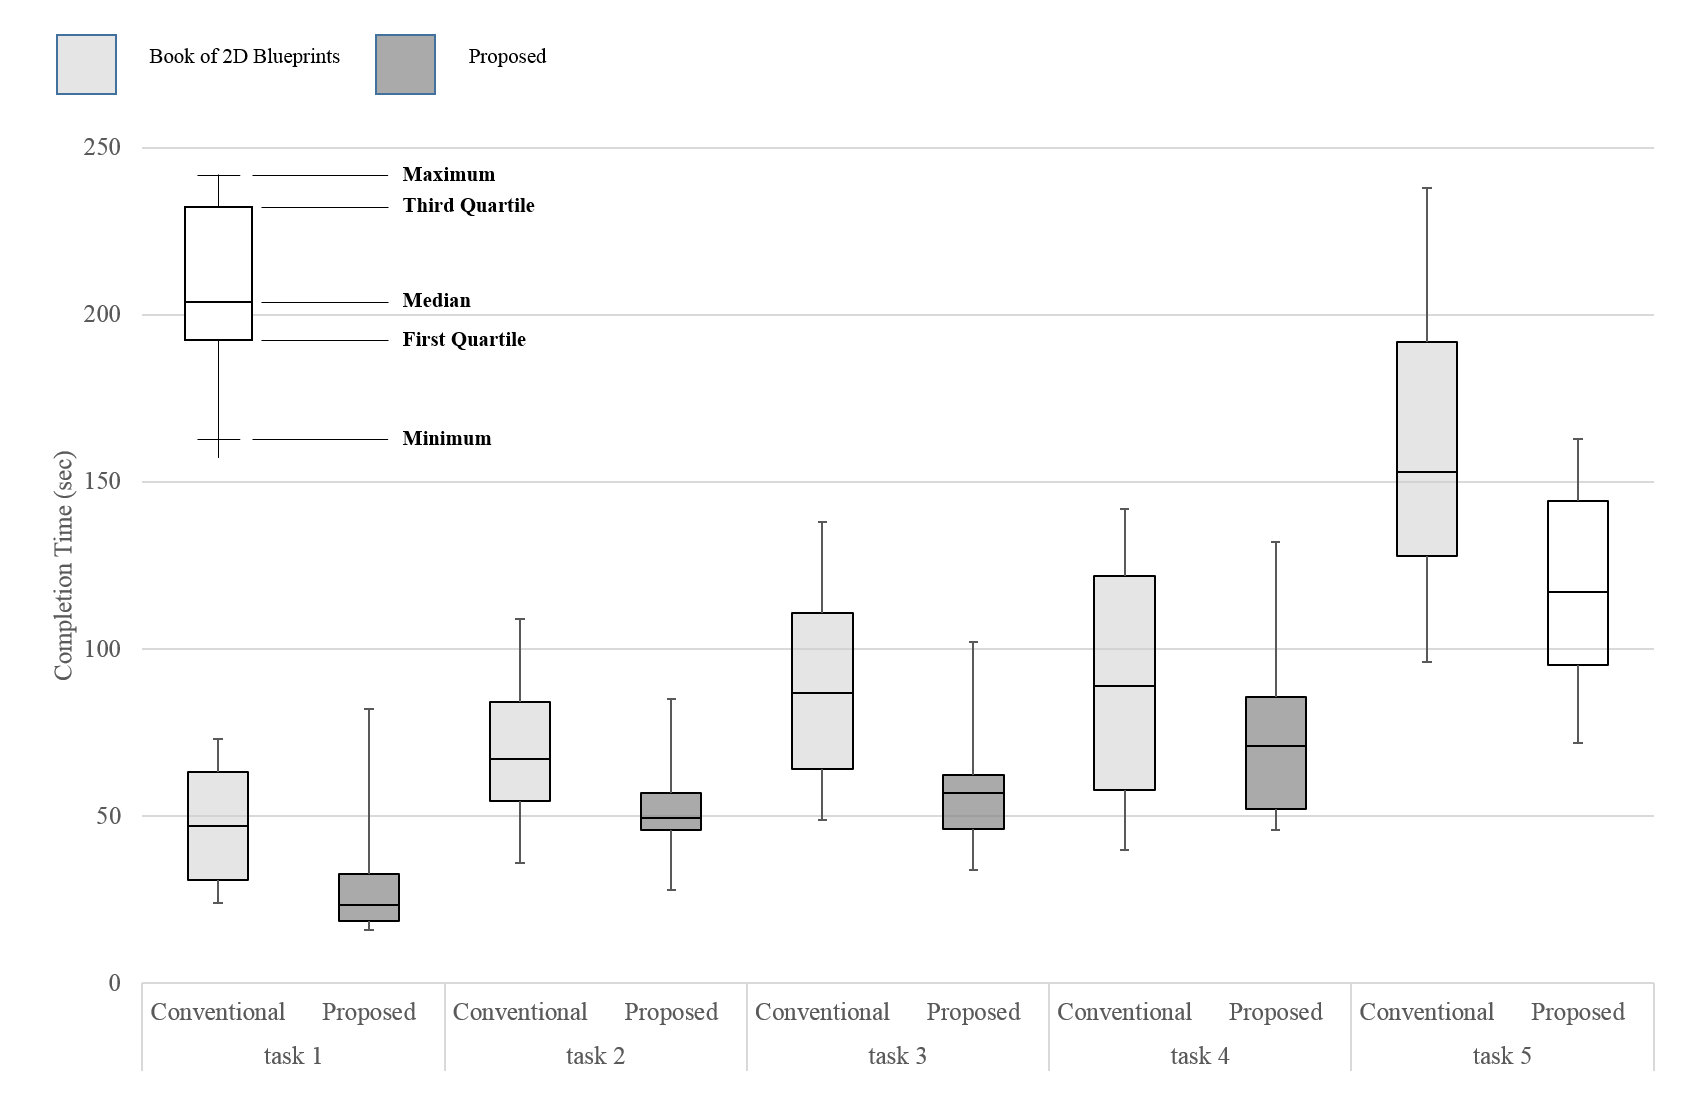
\includegraphics[width=0.8\textwidth, height=7.8cm]{5-Experiments/completion_time}
% \caption{Test completion time}
% \label{fig:completion_time}
% \end{figure*}

% \section{Experiments}
% % \begin{comment}
% 제안하는 시스템의 사용성을 검증하기 위하여 사용자 테스트를 수행하였다. 실험의 설계는 \cite{song_penlight:_2009, yeh_-site_2012}를 참고하여 설계되었다. %완료%


% 실험은 4가지 테스트 시나리오에 대하여 정량적 평가와 정성적 평가를 수행하였다. 그리고 semistructured interview 를 통하여 추가적인 comment와 insight를 얻을 수 있었다.   %수정?%
% % \end{comment}

% %% 번역 원본
% % To verify usability of the proposed system, a user test was executed. The experiment was conducted referring to \cite{song_penlight:_2009, yeh_-site_2012}. We executed a comparison test against conventional 2D drawing based approach, and took questionaire about perceived usefulness and ease of use. Then, through a semistructured interview, additional comments and insight could be gained.

% %% 번역 결과
% % A user test was conducted to verify usability of the proposed system, referring to \cite{song_penlight:_2009, yeh_-site_2012}. We conducted a comparison test against a conventional 2D drawing based approach and circulated questionnaires regarding perceived usefulness and ease of use. Then, additional comments and insight were obtained through semi-structured interviews.


% \subsection{Test Participants}
% % \begin{comment}
% 총 20명의 피실험자(participants)가 실험에 참여하였다.이 중 5명은 여자였고 15명의 남자가 참여했으며, 건축학과 대학원생이었다. 참여자의 나이는 26세부터 43세까지이다(평균 33.6세, SD 4.87세). 이들은 도면에 대한 이해도가 높고 CAD 프로그램에 대한 경험이 많았다. 모두 Kinect 등 제스처 기반 시스템에 대한 경험은 없었다. %완료%
% % \end{comment}

% %% 번역 원본
% % A total of 20 participants joined the experiment. Among them, five were women and 15 were men, they were all graduate school students of the department of architecture. Ages of participants are from 26 to 43 years old (average 33.6 years old, SD of 4.87 years old). They were highly experienced with using and designing blueprints and had a lot of experience in CAD programs. But, they all did not have experience in systems based on gestures like Kinect, and so on.

% %% 번역 결과
% % A total of 20 participants joined the experiment, five women and 15 men, all graduate school students in the department of architecture. Ages of participants ranged from 26 to 43 years (average: 33.6 years, standard deviation: 4.87 years). They were highly experienced in using and designing blueprints and in CAD programs. However, not all had experience in gesture-based systems such as Kinect.

% \subsection{Test Plan}
% % \begin{comment}
% 실험은 \cite{song_penlight:_2009}에서와 같이, 초반 15분 동안 demonstration session을 진행하였다. demonstration session 동안, 전체 시나리오에 대한 비디오를 보여준 후, 제안하는 시스템의 사용 방법에 대하여 설명하고, 나머지 시간동안 실제로 사용해볼 수 있도록 하였다. 이후에 비교 실험과  사용성 평가를 실시하였다. 비교 실험은 \cite{yeh_-site_2012}와 마찬가지로 제안하는 시스템과 대조군 시스템 사이의 비교실험을 적용하여 몇 가지 과제를 수행하도록 하고 수행 시간을 비교하였다. 대조군 시스템은 건축 도면 묶음을 이용하여 주어진 과업(task)을 수행하도록 하였고, 4번 과업은 모델에 접근이 필요하기 때문에 노트북에서 \textit{SketchUp} 사용하도록 하였다. \textit{SketchUp} 프로그램의 제어에 사용된 인터페이스는 키보드와 마우스를 제공하였다. 사용성 평가는 비교 실험 후에 \cite{davis_perceived_1989}의 설문을 수행하고 간단한 코멘트를 작성하도록 하였다.
% % \end{comment}
% %% 번역 원본
% % In the experiment, a demonstration session was done for the first 15 minutes like \cite{song_penlight:_2009}. During the demonstration session, after showing a video about all the scenarios, a usage tutorial of the proposed system was explained, and for the of the rest time, the system was used by the participants. Then, the comparison experiment and usability evaluation were conducted. In the comparison experiment, like \cite{yeh_-site_2012}, by applying the comparison experiment between the proposed system and a comparison group system, a few assignments were executed and their execution times were compared. In the comparison group system, using a bundle of construction blueprints, several given tasks were executed. Since the fourth task was necessary for accessing the models, \textit{SketchUp} was made to be used on a laptop. For the usability evaluation, a survey based on \cite{davis_perceived_1989} was conducted after the comparison experiment and participants wrote down simple comments about their experience.

% %% 번역 결과
% % In the experiment, a demonstration session was conducted for the first 15 minutes, as in \cite{song_penlight:_2009}. During the demonstration session, after a video describing all of the scenarios was shown, a usage tutorial of the proposed system was explained, and then the system was used by the participants for the remaining time. Then, the comparison experiment and usability evaluation were conducted. In the comparison experiment, as in \cite{yeh_-site_2012}, a few assignments were executed and their execution times were compared by conducting the comparison experiment between the proposed system and a comparison group system. Several given tasks were executed in the comparison group system, using a number of construction blueprints. Since the fourth task was necessary for accessing the models, SketchUp was installed for use on a laptop. For the usability evaluation, a survey based on \cite{davis_perceived_1989} was conducted after the comparison experiment, and participants wrote simple comments regarding their experience.

% %\textcolor{red}{\textit{SketchUp} 프로그램의 제어에 사용된 인터페이스는 키보드와 마우스를 제공하였다.}

% %%%%%%%%%%%%%%%%%%%%%%%%%%%%%%%%%%%%%%%%%%%%%%%%%%%%%%%%%%%%%%%%%%%%%%%%%%%%%%%%%%%%%%%%

% \subsection{Test Tasks}
% % \begin{comment}
% 비교 실험에 수행된 과업은 \cite{yeh_-site_2012}와 유사하게 설계하여 실제 건축 환경에서 문제가 되는 task를 반영하였다. 이는 건축 현장에서 건축물의 정보를 획득하고 이를 다시 건축 모델에 반영하는 일련의 과정을 반영하고 있다. 세부적인 task는 아래와 같다. 각 task는 독립적으로 수행되었으며, 새로운 task 수행 전에 5분 간의 휴식 시간을 제공하였다. 실험은 이러한 각 task의 수행 시간을 측정하였다. 
% \begin{enumerate}
% \item Exploration: 3차원 모델을 돌려보고 특정 뷰에 있는 특징 발견하기
% \item Query: 특정 층의 특정 평면도 획득
% \item Legend: 건축물의 평면도에서 특정 구조물의 dimension 획득
% \item Modify: 건축물의 평면도에서 특정 구조물을 다른 위치로 이동됨을 표시
% \item Discussion: 원격의 관리자와 건축물의 특정 위치의 이슈에 대하여 의견 교환
% \end{enumerate}
% % \end{comment}

% %% 번역 원본
% % The tasks conducted in the comparison experiment was designed similar to \cite{yeh_-site_2012}, and was done to reflect real construction environments. The experiment allowed a number of ways that information of buildings could be acquired and reflected on construction models again. Details of the tasks are as follows. Each task was executed independently, and a 5-minute break time was provided before the task execution. The experiment measured the execution time of each task.

% %% 번역 결과
% % The tasks executed in the comparison experiment were designed, similarly to those in \cite{yeh_-site_2012}, to reflect real construction environments. The experiment allowed a number of ways by which building information could be acquired and reflected in construction models. Details of the tasks are as follows. Each task was executed independently, and a 5 minutes break was provided before task execution. The experiment measured the execution time of each task.

% % \begin{enumerate}
% % \item Exploration: Viewing a 3D model while turning it around, and finding out characteristics in a special view
% % \item Query: Acquisition of a special floor plane in a special layer
% % \item Legend: Acquisition of a dimension of a special structure on a floor plane of a building
% % \item Modify: Mark of moving of a special structure into other location on a floor plane of a building
% % \item \modified{Discussion: Discuss with a constructional manager in remote place about on-site issue}

% % \end{enumerate}

% % \begin{enumerate}
% % \item Exploration: Viewing a 3D model while turning it and determining characteristics in a specific view
% % \item Query: Acquisition of a special floor plane in a specific layer
% % \item Legend: Acquisition of a dimension of a specific structure on a floor plane of a building
% % \item Modify: Marking the moving of a specific structure into another location on a floor plane of a building.
% % \item \modified{Discussion: Discussion with a constructional manager in remote place about on-site issue}
% % \end{enumerate}


% %%%%%%%%%%%%%%%%%%%%%%%%%%%%%%%%%%%%%%%%%%%%%%%%%%%%%%%%%%%%%%%%%%%%%%%%%%%%%%%%%%%%%%%%

% \subsection{Test Results}
% % \begin{comment}
% 실험의 결과는 비교 실험의 결과와 사용성 테스트의 결과를 나누어 설명한다.
% % \end{comment}

% % Test results are explained and divided into an experiment result and usability test result.

% \subsubsection{Comparison Test}
% % \begin{comment}
% \cite{yeh_-site_2012}에서는 과업의 수행 시간과 성공률을 나누어 측정하였다. 하지만 우리의 실험에서는 모두 성공하였으므로 수행 시간만을 보고 한다. 수행 시간은 표 \ref{tab:comparison}에서 보듯이 전체적으로 제안하는 방법이 2D 도면 기반의 방법에 비하여 월등한 속도를 보여주었다. 4개의 과업 모두 t-test 결과 positive 하고 통계적으로 상당한(significant) 차이가 났다(p \textless 0.05). 하지만, 그림 \ref{fig:completion_time}에서 보는 것과 같이, 제안하는 방법은 굉장히 낮은 Median과 First/Third Quartile 값을 보여주지만 Maximum 값의 경우 2D drawing 방법보다 크게 나오는 경우들이 발생하였다. 이는 3차원 모델을 조작하는 과정에서 gestural interface가 익숙하지 못하여 시간이 오래 걸린 표본이 간혹 발생한 것을 나타낸다. 이러한 문제는 새로운 인터페이스에 적응하는 과정에서 발생하는 문제로 longitudinal study를 추가로 수행하여 장기적 관점에서 인터페이스의 성능을 측정하는 것이 필요할 것으로 보인다. 하지만 낮은 quartile value를 볼 때 전체적인 표본들의 수행 속도는 큰 차이가 나지 않고 빠른 것을 볼 수 있었다. 기존 방법에 비하여 숙련자와 비숙련자 간의 속도 차이가 적음을 알 수 있다. 
% 특히, Discussion 작업의 경우에는 원격지에서 눈에 보이는 것이 없이 커뮤니케이션하는 것에 비하여 on-site에서 직접 이슈를 보면서 커뮤니케이션하기 때문에 수행시간의 차이가 크게 나타났으며, 커뮤니케이션 과정에서 좀 더 자세한 discussion이 이루어졌다. 하지만, 화면이 작기 때문에 아이템의 터치 과정에서 에러가 자주 발생하였고, 선택된 아이템의 visual feedback이 부족하여 작업 과정에서 에러가 자주 발생하였다. 이러한 부분은 개선이 필요하였다. 

% 이렇게 제안하는 방법은 기존의 2D 도면책 방법에 비하여 작업의 효율성을 높여주었다. 특히, 3차원 건축 데이터를 현장에서 자연스럽게 navigation이 가능하였고, 협업에 편리함을 제공함을 확인할 수 있었다.
% % \end{comment}

% \renewcommand{\multirowsetup}{\centering}  % 기본값은 \raggedright
% \renewcommand{\arraystretch}{1.2} 

% \begin{table}[!b]
%   \centering
%   \begin{tabular}{|c|c|rrr|}
%     \hline
%     \multicolumn{1}{|p{0.11\columnwidth}}{} &
%     \multicolumn{1}{p{0.21\columnwidth}}{} &
%     \multicolumn{1}{|p{0.15\columnwidth}}{\centering\tabhead{Mean (s)}} &
%     \multicolumn{1}{p{0.15\columnwidth}}{\centering\tabhead{SD (s)}} &
%     \multicolumn{1}{p{0.15\columnwidth}|}{\centering\tabhead{t}} \\
%     \hline
% 	\multirow{2}*{Task 1} & Conventional & 47.10 & 17.54 & \multirow{2}*{7.76}\\
%       & Proposed & 28.75 & 16.08 & \\
%     \hline
% 	\multirow{2}*{Task 2} & Conventional & 68.45 & 20.37 & \multirow{2}*{8.36}\\
%       & Proposed & 51.10 & 12.34 & \\
%     \hline
% 	\multirow{2}*{Task 3} & Conventional & 89.20 & 28.81 & \multirow{2}*{9.44}\\
%       & Proposed & 57.60 & 16.42 & \\
%     \hline
% 	\multirow{2}*{Task 4} & Conventional & 91.00 & 34.33 & \multirow{2}*{5.78}\\
%       & Proposed & 70.95 & 22.32 & \\
%     \hline
%   \multirow{2}*{Task 5} & Conventional & 161.40 & 118.55 & \multirow{2}*{13.41}\\
%       & Proposed & 118.55 & 29.39 & \\
%     \hline
%   \end{tabular}
%   \caption{Comparison Result}
%   \label{tab:comparison}
% \end{table}

% % In \cite{yeh_-site_2012}, the execution time and success rate of tasks were measured separately. But, because our experiment succeeded in all tasks, only the execution time is reported. In the execution time, the proposed method showed excellent speed compared to the method based on 2D blueprints(see Table \ref{tab:comparison}). Four tasks all represented positive t-test results and significant differences statistically (p $\textless$ 0.05). However, as seen from Figure \ref{fig:completion_time}, although the proposed method showed extremely low values of median and first/third quartile, in case of maximum values, some cases show bigger values than 2D drawing cases. 
% % This means that since gestural interfaces were unfamiliar in the course of manipulating 3D models, a long time-taking specimens sometimes occurred. This problem is a problem occurring in the course of applying to new interfaces. So, it seems that to measure interface performances from a long time viewpoint is necessary by conducting a longitudinal study additionally. But, when seeing low quartile values, overall execution speeds were seen to be fast without significant differences. Compared to existing methods, it can be known that differences of speeds between the skilled and the unskilled are small.

% % Especially for task 5, conventional methods have to communicate without visible materials present, but proposed system can communicate with visual information concerning on-site issues. So, we can reduce completion time. Also, it offers more details in communication. Mobile devices also have problems since the tiny touch-screen offers little visual feedback. Touch errors can also occur while performing task in the mobile personal workspace. As these results show, the proposed system offers a more efficient interface rather than relying on conventional books of 2D blueprints. Understanding and access to content is faster and offers a natural navigation for 3D architectural data in the construction space as well as offering convenient remote collaboration between remote construction sites.




% \subsubsection{Usability Test}
% % \begin{comment}
% 사용성은 demonstration 세션과 비교 실험이 모두 완료된 후에 참여자들에게 설문을 통하여 수행되었다. 설문은 \cite{perlman_user_2011}를 기반으로 수행되었으며, 7-point Likert scale로 평가되었다. 
% 평가는 Task 1~4에서의 Shared workspace 에 대한 사용성과 Task 5의 Shared와 Personal workspace의 혼합 시스템에 대하여 각각 수행되었다.
% % \end{comment}

% % Usability was conducted through a survey after the demonstration session and the comparison experiment were finished. The survey was executed on the basis of \cite{perlman_user_2011} and was evaluated by 7-point Likert scale. \modified{The target system for the survey is shared workspace only(task 1$\sim$4) and combined workspace(task 5).}

%  \begin{figure}[b!]
% \centering
% 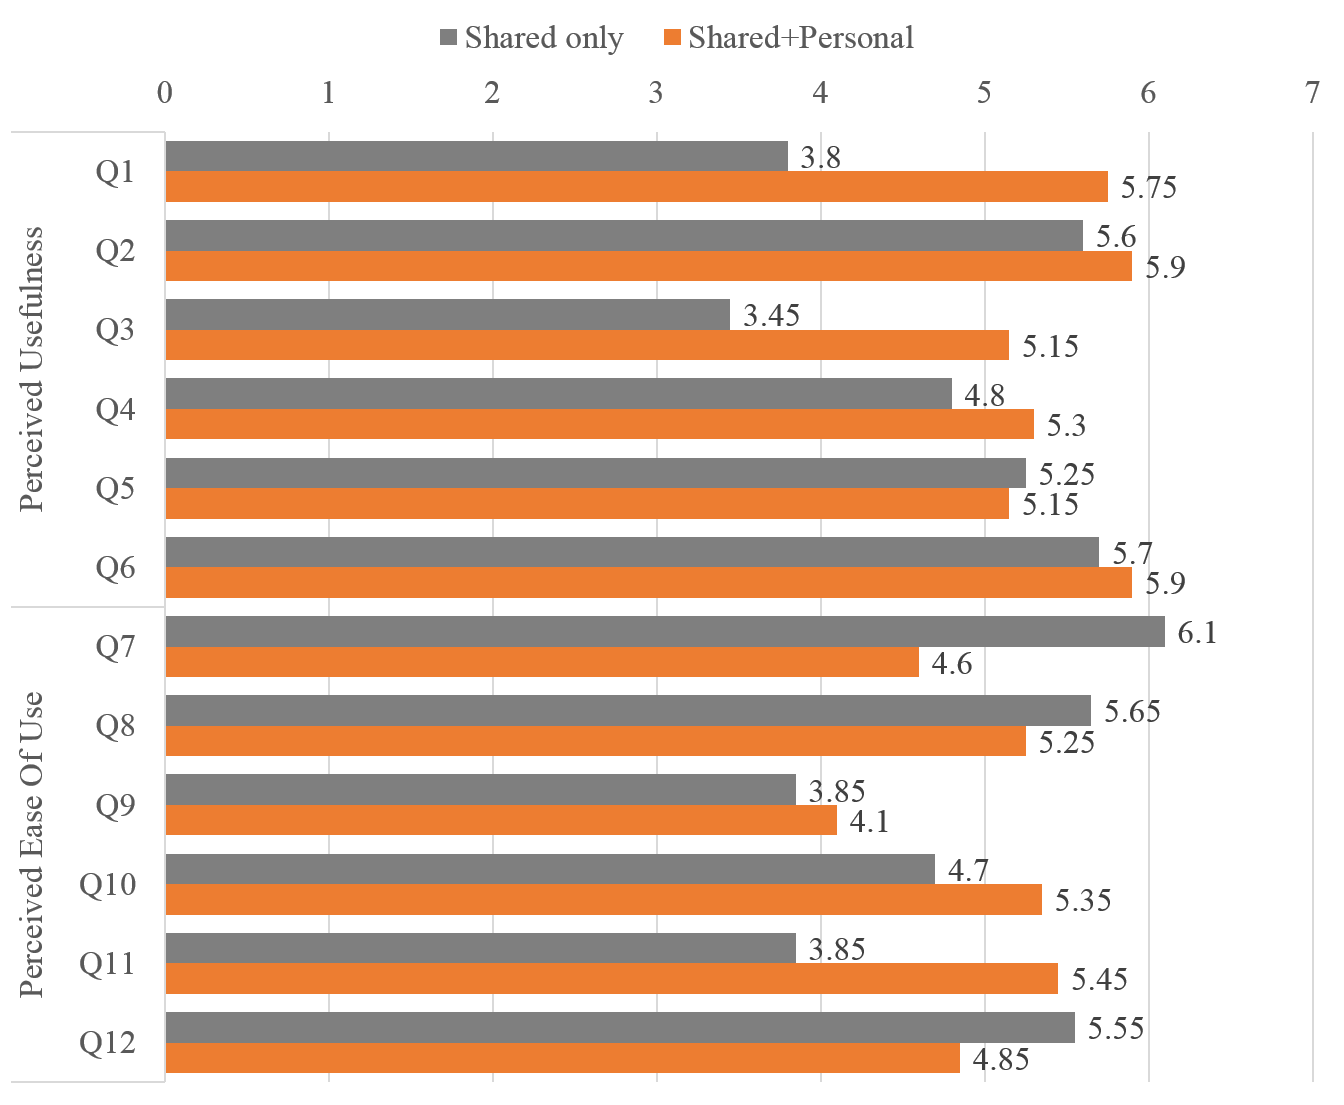
\includegraphics[width=1.0\columnwidth, height=5.5cm]{5-Experiments/pueu}
% \caption{Perceived Usefulness and Ease of Use}
% \label{fig:pueu}
% \end{figure}

% % \begin{comment}
% 그림 \ref{fig:pueu}에서 보듯이 전체적으로 평균에 비하여 높은 점수를 받았다. 특히 usefulness 항목에서는 Q2의 job performance에 관련된 내용과 Q6의 usefulness 항목이 높은 점수를 받아 제안하는 시스템이 작업의 효율을 높여줄 것이라는 의견이 많았다. 하지만, Q3의 점수가 낮게 나온 것으로 보아 생산성의 향상으로 연결되지는 않을 것으로 예상되었다. ease of use 항목에서는 Q7과 Q12가 높은 점수가 나온 것으로 보아 시스템이 쉽게 배우고 사용하기가 편리하다는 평가가 많았다. 하지만, Q9와 Q11의 점수가 낮은 것으로 보아 아직 시스템에 대한 파악이 다 되지 못하여 이해가 어려웠음을 알 수 있었다.
% 두 시스템 간의 비교를 보면, 전체적으로 combined workspace(combined using shared workspace and mobile personal workspace)에서는 usefulness 가 높게 측정된 반면, ease of use 항목은 점수가 낮았다. 특히, Q1과 Q3 항목에서 큰 차이를 보여주어, combined workspace에서 productivity가 높고 빠르게 task를 완료할 수 있을 것으로 기대되었다. 이는 construction 과정에서 발생되는 이슈에 대하여 빠르고 효율적으로 discussion 이 가능하기 때문으로 분석되었다. 반면, 모바일 시스템에 대한 학습이 필요하므로 전체적으로 Ease of Use 항목은 점수가 낮게 측정되었다.
% % \end{comment}

% % As seen in Figure \ref{fig:pueu}, overall, high scores were gained compared to the average. Especially, in the usefulness, there were lots of opinions that the proposed system would heighten work efficiency since the contents related with job performance of Q2 and the item of usefulness of Q6 gained high scores. Nonetheless, from the low score of Q3, it was predicted that it would not be linked with productivity increase. In ease of use, from seeing high scores of Q7 and Q12, there were a lot of evaluations that the system was easy to learn and convenient to use. However, from seeing low scores of Q9 and Q11, it was known that the understanding was difficult caused from insufficient grasping of the system.

% % In regards to the comparison between shared workspace only against combined workspace (combine using shared workspace and mobile personal workspace), combined workspace is perceived as higher usefulness and lower ease of use. Especially Q1 and Q3 show high differences, because the combined workspace offers efficient and rapid discussion mechanisms, so it is shown to support higher productivity and expect a fast task completion. In contrast, it has to be learnt to use on mobile applications. Overall score of Ease of Use for combined workspace showed a larger gain over a shared only workspace.


% \subsubsection{Discussion}
% % \begin{comment}
% 평가 중에 나왔던 몇 가지 코멘트 등을 통하여 시스템에 대한 주관적 평가들을 받을 수 있었다. 주로 많이 나왔던 코멘트는 현재 시스템의 하드웨어의 복잡성에 대한 의견이 많았다. 현재는 노트북에 연결하여 사용하기 때문에 시스템과 별도로 노트북이 필요하고, 연결선으로 인해 복잡하다는 반응이 많았다. 이러한 문제는 향후 Mobile Depth Camer 기술을 적용하여 Android나 iOS와 같은 모바일 버전으로 발전시켜 나가면서 해결할 수 있을 것으로 기대된다. 또한, 현재 적용된 Portable Projector에서도 화면의 FoV(Field-of-View)가 작고 밝기가 낮아서 외부 환경에서 사용하기에 적합하지 않았다. 이 또한 projector 기술의 발전과 함께 해결될 수 있을 것으로 기대된다. 마지막으로 현재 사용되고 있는 Leap Motion 기기를 이용한 손 인식 방법이 정확도는 매우 높으나, 시스템과 별도로 설치를 해야하는 문제가 있기 때문에 거추장스럽다는 의견이 많았다. 이는 시스템에 integrate 된 depth camera를 이용하여 인식함으로써 시스템을 단순화하여 제공할 수 있을 것으로 기대된다. 
% 그리고 Mobile Personal Workspace에서는 기기의 크기가 작기 때문에 세밀한 Component의 터치가 부정확하고, 선택된 Component에 대한 Visual feedback이 부족하기 때문에 작업 과정에서 오류가 자주 일어났다. 이러한 문제를 해결하기 위하여 \cite{vogel_shift:_2007}와 같은 터치 인터페이스의 개선이 적용된다면 더 높은 사용성을 제공할 수 있을 것이다.
% % \end{comment}

% % Through several comments during the evaluation, subjective evaluations of the system could be observed. Comments which came out mostly were opinions about complexity of hardware of the present system. Presently, because testing Port3DAr was used with connected laptops, there were a lot of responses that laptops are necessary apart from the system and it was complex due to connection lines. These problems can be expected to be settled from developing the system into a mobile version on smart devices using Android or iOS platforms. 
% % In addition, in the presently applied portable projector, because the Field-of-View of a screen was small and the brightness was low, it was not proper to use in external environments. It is also expected that these can be solved with the development of projector technology. Lastly, though the hand recognition method using leap motion devices presently used is high in accuracy, there were lots of opinions that it is burdensome due to the installation apart from the system. It is anticipated that the solution can be provided from the simplification of the system, by recognizing hands using a depth camera which is integrated into the system.
% % Also, for mobile personal workspaces, there are frequent errors because the device is too small to select items and there is a lack of visual feedback. To improve these problems, we implement an enhancement technique for mobile touch devices similar to \cite{vogel_shift:_2007}.
% %그리고 Mobile Personal Workspace에서는 기기의 크기가 작기 때문에 세밀한 Component의 터치가 부정확하고, 선택된 Component에 대한 Visual feedback이 부족하기 때문에 작업 과정에서 오류가 자주 일어났다. 이러한 문제를 해결하기 위하여 \cite{vogel_shift:_2007}와 같은 터치 인터페이스의 개선이 적용된다면 더 높은 사용성을 제공할 수 있을 것이다.
